%% Mark to describe method used to tag and time articles 
\documentclass[a4paper, 12pt]{article} 
\usepackage{amsmath, amssymb, color, graphicx, enumitem}
\usepackage{fullpage} %smaller margins
\usepackage{hyperref} % hyperlinks
\usepackage{url} %sensible urls
\usepackage{todo} %creates todo in margins
\usepackage{booktabs} % better looking tables


%font, libertine
\usepackage{libertine}
%word spacing
\usepackage{microtype}
%all equations get full space
\everymath{\displaystyle}

%columns separate and line
\usepackage{multicol}
\setlength{\columnsep}{1.5cm}
\setlength{\columnseprule}{0.2pt}

%environment
\newcommand{\tab}{\phantom{ssss}}

%=======================Shortcuts==============================================
%useful shortcuts
\def\R{\ensuremath{\mathbb{R}}} %\ensuremath adds math mode, if forgotten
\def\Q{\ensuremath{\mathbb{Q}}}
\def\N{\ensuremath{\mathbb{N}}}
\def\Z{\ensuremath{\mathbb{Z}}}
\def\C{\ensuremath{\mathbb{C}}}

%shorcuts with arguments
\newcommand{\abs}[1]{\left\vert#1\right\vert} %nice absolute values
\newcommand{\bt}[1]{\textbf{#1}} %bold
\newcommand{\eq}[1]{\begin{align*}#1\end{align*}} %aligned equations
\newcommand{\norm}[1]{\left\lVert#1\right\rVert} %vector norm
\newcommand{\notimplies}{% does not imply
    \mathrel{{\ooalign{\hidewidth$\not\phantom{=}$\hidewidth\cr$\implies$}}}}
\renewcommand{\eq}[1]{\begin{align*}#1\end{align*}} %aligned equations


%colors
\definecolor{javagreen}{rgb}{0.25,0.5,0.35} %dark green color
\definecolor{lightblue}{rgb}{0.149,0.545,0.824} %solarized blue
\definecolor{sred}{rgb}{0.863, 0.196, 0.184} %solarized red

\newcommand{\blue}[1]{{\leavevmode\color{lightblue}{#1}}} %solarized blue 
\newcommand{\green}[1]{{\leavevmode\color{javagreen}{#1}}} %command for green
\newcommand{\red}[1]{{\leavevmode\color{sred}{#1}}} %solarized red
\newcommand{\gray}[1]{{\leavevmode\color[gray]{0.5}{#1}}} %gray text

%==TODO==
% boxes?
%checkout: http://blog.rtwilson.com/my-latex-preamble/

\title{}
\date{}
% ========================== Tips =============================================
%part
    %section, sub, sub

%\begin{enumerate}[resume] %continues counting

% Piecewise Function
%\begin{displaymath}
%   f(x) = \left\{
%     \begin{array}{lr}
%       1 & : x \in \mathbb{Q}\\
%       0 & : x \notin \mathbb{Q}
%     \end{array}
%   \right.
%\end{displaymath} 

% Images
% \includesgraphics{image.png}

% Tables
%\begin{tabular}{llr}
%    \toprule
%    first name & last name & $\chi$\\
%    \midrule
%    second & last & first \\
%    \bottomrule
%\end{tabular}

% ========================== End of Tips ======================================

% figures path
\graphicspath{{figures/}}

\begin{document}
\begin{center}
\section*{Methods}
\end{center}

\subsection*{Historical Thesaurus}

Categories, third level.
    * total is 235,000 entry categories
* The Thesaurus was compiled over a period of 44 years
* While the OED is a hugely rich resource for studying the histories of individual words, there was no parallel resource for studying the history of concepts as they are expressed in word
* classificatory principle on which the Thesaurus is based: a progression from the most general terms to the most specific.
* from editor notes: "A scroll through a section such as Food or Inhabiting/dwelling illustrates how far people’s lives have changed over time."


\subsection*{Tagging Topics}

Typical usage online allows you to explore words inside a category, we'll flip that so we can explore categories of text.

* taking the category by the word appears
* by taking all the categories along with a count, we can get a list of potential category tags


\subsection*{Application to Wikipedia}

We use this idea not only to tag categories to obtain a view of the areas of knowledge through article titles, 
but we also obtain a historical pesepctive of wikipedia.

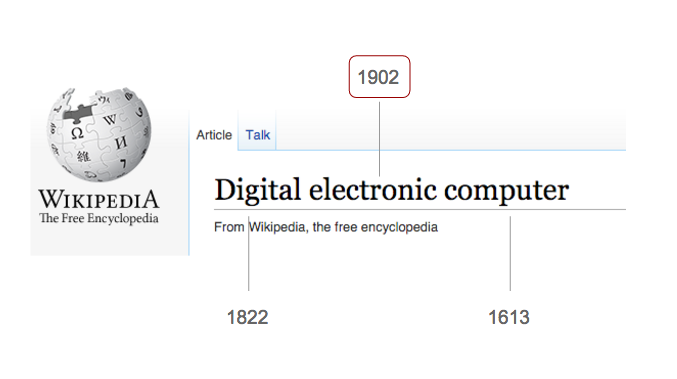
\includegraphics[width=\textwidth]{title_dates}  
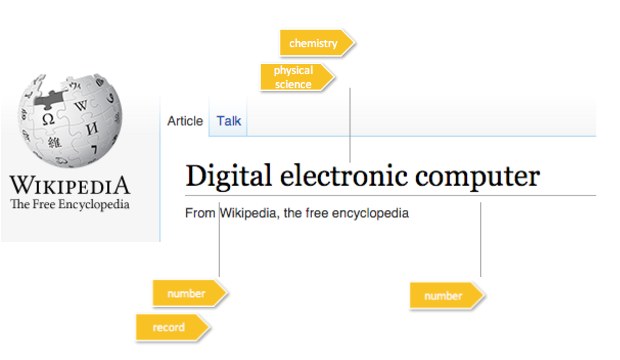
\includegraphics[width=\textwidth]{title_tags}  

\end{document}

